\documentclass[12pt]{article}
\usepackage[left=1cm, right=1cm, top=2cm,bottom=1.5cm]{geometry} 

\usepackage[parfill]{parskip}
\usepackage[utf8]{inputenc}
\usepackage[T2A]{fontenc}
\usepackage[russian]{babel}
\usepackage{enumitem}
\usepackage[normalem]{ulem}
\usepackage{amsfonts, amsmath, amsthm, amssymb, mathtools}
\usepackage{tabularx}
\usepackage{hhline}

\usepackage{accents}
\usepackage{fancyhdr}
\pagestyle{fancy}
\renewcommand{\headrulewidth}{1.5pt}
\renewcommand{\footrulewidth}{1pt}

\usepackage{graphicx}
\usepackage[figurename=Рис.]{caption}
\usepackage{subcaption}
\usepackage{float}

%%Наименование папки откуда забирать изображения
\graphicspath{ {./images/} }

%%Изменение формата для ввода доказательства
\renewcommand{\proofname}{$\square$  \nopunct}
\renewcommand\qedsymbol{$\blacksquare$}

%%Изменение отступа на таблицах
\addto\captionsrussian{%
	\renewcommand{\proofname}{$\square$ \nopunct}%
}
%% Римские цифры
\newcommand{\RN}[1]{%
	\textup{\uppercase\expandafter{\romannumeral#1}}%
}

%% Для удобства записи
\newcommand{\MR}{\mathbb{R}}
\newcommand{\MC}{\mathbb{C}}
\newcommand{\MQ}{\mathbb{Q}}
\newcommand{\MN}{\mathbb{N}}
\newcommand{\MTB}{\mathbb{T}}
\newcommand{\MTI}{\mathbb{I}}
\newcommand{\MI}{\mathrm{I}}
\newcommand{\MJ}{\mathrm{J}}
\newcommand{\MH}{\mathrm{H}}
\newcommand{\MT}{\mathrm{T}}
\newcommand{\MU}{\mathcal{U}}
\newcommand{\MV}{\mathcal{V}}
\newcommand{\MB}{\mathcal{B}}
\newcommand{\MW}{\mathcal{W}}
\newcommand{\ML}{\mathcal{L}}
\newcommand{\VN}{\varnothing}
\newcommand{\VE}{\varepsilon}

\theoremstyle{definition}
\newtheorem{defn}{Опр:}
\newtheorem{rem}{Rm:}
\newtheorem{prop}{Утв.}
\newtheorem{exrc}{Упр.}
\newtheorem{lemma}{Лемма}
\newtheorem{theorem}{Теорема}
\newtheorem{corollary}{Следствие}

\newenvironment{cusdefn}[1]
{\renewcommand\thedefn{#1}\defn}
{\enddefn}

\DeclareRobustCommand{\divby}{%
	\mathrel{\text{\vbox{\baselineskip.65ex\lineskiplimit0pt\hbox{.}\hbox{.}\hbox{.}}}}%
}
%Короткий минус
\DeclareMathSymbol{\SMN}{\mathbin}{AMSa}{"39}
%Длинная шапка
\newcommand{\overbar}[1]{\mkern 1.5mu\overline{\mkern-1.5mu#1\mkern-1.5mu}\mkern 1.5mu}
%Функция знака
\DeclareMathOperator{\sgn}{sgn}

%Функция ранга
\DeclareMathOperator{\rk}{\text{rk}}

%Обозначение константы
\DeclareMathOperator{\const}{\text{const}}

\DeclareMathOperator*{\dsum}{\displaystyle\sum}
\newcommand{\ddsum}[2]{\displaystyle\sum\limits_{#1}^{#2}}

%Интеграл в большом формате
\DeclareMathOperator{\dint}{\displaystyle\int}
\newcommand{\ddint}[2]{\displaystyle\int\limits_{#1}^{#2}}
\newcommand{\ssum}[1]{\displaystyle \sum\limits_{n=1}^{\infty}{#1}_n}

\newcommand{\smallerrel}[1]{\mathrel{\mathpalette\smallerrelaux{#1}}}
\newcommand{\smallerrelaux}[2]{\raisebox{.1ex}{\scalebox{.75}{$#1#2$}}}

\newcommand{\smallin}{\smallerrel{\in}}
\newcommand{\smallnotin}{\smallerrel{\notin}}

\newcommand*{\medcap}{\mathbin{\scalebox{1.25}{\ensuremath{\cap}}}}%
\newcommand*{\medcup}{\mathbin{\scalebox{1.25}{\ensuremath{\cup}}}}%

\makeatletter
\newcommand{\vast}{\bBigg@{3.5}}
\newcommand{\Vast}{\bBigg@{5}}
\makeatother

%Промежуточное значение для sup\inf, поскольку они имеют разную высоту
\newcommand{\newsup}{\mathop{\smash{\mathrm{sup}}}}
\newcommand{\newinf}{\mathop{\mathrm{inf}\vphantom{\mathrm{sup}}}}

%Скалярное произведение
\DeclarePairedDelimiterX{\inner}[2]{\langle}{\rangle}{#1, #2}

%Подпись символов снизу
\newcommand{\ubar}[1]{\underaccent{\bar}{#1}}

%% Шапка для букв сверху
\newcommand{\wte}[1]{\widetilde{#1}}

%%Функция для обозначения равномерной сходимости по множеству
\newcommand{\uconv}[1]{\overset{#1}{\rightrightarrows}}

%%Функция для обозначения нижнего и верхнего интегралов
\def\upint{\mathchoice%
	{\mkern13mu\overline{\vphantom{\intop}\mkern7mu}\mkern-20mu}%
	{\mkern7mu\overline{\vphantom{\intop}\mkern7mu}\mkern-14mu}%
	{\mkern7mu\overline{\vphantom{\intop}\mkern7mu}\mkern-14mu}%
	{\mkern7mu\overline{\vphantom{\intop}\mkern7mu}\mkern-14mu}%
	\int}
\def\lowint{\mkern3mu\underline{\vphantom{\intop}\mkern7mu}\mkern-10mu\int}


\begin{document}
\lhead{Математический анализ - \RN{3}}
\chead{Шапошников С.В.}
\rhead{Лекция - 15}
\section*{Степенные ряды}
Пусть у нас есть некоторая функция $f(x)$, очень часто хочется её представить в виде суммы простых функций (в некотором роде разложить по базису функций $\{\varphi_n(x)\}_{n = 0}^{\infty}$):
$$
	f(x) = \ddsum{n = 0}{\infty}c_n \varphi_n(x)
$$
Поскольку функция сложная, то сумма будет до бесконечности. Встает вопрос, что за разумные $\varphi_n(x)$ могут здесь использоваться? Первое, что приходит на ум - многочлены $\Rightarrow$ разумно рассматривать следующую систему: 
$$
	\{1, x, x^2, \dotsc, x^n, \dotsc\}
$$
Вместо такой системы можно рассматривать систему со сдвигом:
$$
	\{1, x - x_0, (x - x_0)^2, \dotsc, (x - x_0)^n, \dotsc\}
$$
Но всегда можно сделать обратный сдвиг, поэтому не будем её рассматривать (будем смотреть системы с центром в нуле). Мы хотим уметь раскладывать любую функцию по таким системам. Рассмотрим следующий пример:
$$
	f(x) = \dfrac{1}{1+x^2}, \, f(x) \in C^{\infty}(\MR)
$$
$f(x)$ это гладкая, хорошая функция на всём $\MR$, попробуем разложить её в ряд:
$$
	f(x) = 1 - x^2 + x^4 - \dotsc  = \ddsum{n = 0}{\infty}(-1)^n x^{2n}, \, |x| < 1
$$
Это обычная геометрическая прогрессия, но такой ряд сходится только лишь при $|x|<1$, при этом сама функция $f(x)$ является бесконечно гладкой на всем $\MR$. Проблема заключается в том, что у этой функции на комплексной плоскости есть особенности: $x = \pm i$. 
\begin{figure}[H]
	\centering
	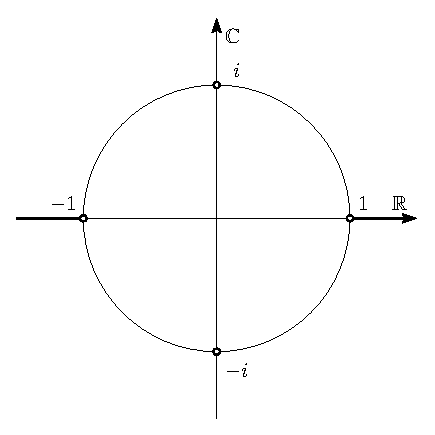
\includegraphics[width=0.3\textwidth]{MA3L15_1.eps}
	\label{MA3L15_1}
	\caption{Круг сходимости у ряда $\ddsum{n = 0}{\infty}(-1)^n x^{2n}$.}
	\label{fig:разложение функции)}
\end{figure}

Таким образом, нам разумно рассматривать разложение в степенные ряды в $\MC$.
\begin{defn}
	Ряд вида $\ddsum{n = 0}{\infty}c_n (z - z_0)^n$ называется \uwave{степенным рядом с центром в} $z_0$, где $\forall n , \, c_n,z, z_0 \in \MC$.
\end{defn}
Далее везде считаем, что $z_0 = 0$.
\newpage

\subsection*{Комплексные числа}
Как уже проходили на алгебре, будем рассматривать комплексные числа следующим образом: 
$$
	\forall z \in \MC, \, z = x + iy 	
$$ 
В комплексной плоскости топология наследуемая метрикой (даже нормой) $\MR^2$:
$$
	\forall z \in \MC, \, |z| = \rho(z,0) = \sqrt{x^2 + y^2}, \, \rho(z_1,z_2) = \sqrt{(x_1 - x_2)^2 + (y_1 - y_2)^2}
$$ 
Сходимость в $\MC$ задается этой же метрикой: $(\MC, \rho)$ - метрическое пространство.
\begin{defn}
	Последовательность $\{z_n\}$ сходится к $z\colon z_n \to z$, если $\rho(z_n,z) \to 0$.
\end{defn}
Дифференцируемость будет определяться в чем-то сложнее, в чем-то проще случая для вещественных пространств. Пусть есть функция в комплексозначной плоскости:
$$
	f \colon \MC \to \MC \longleftrightarrow g \colon \MR^2 \to \MR^2
$$
Ей будет соответствовать некоторая функция $g$ из $\MR^2$ в $\MR^2$. Хотелось бы понять, как будет связано комплексное дифференцирование с вещественным. 

\subsection*{Комплексное дифференцирование}
\begin{defn}
	Функция $f(z)$ - $\MC$-\uwave{дифференцируема в} $z_0$, если существует предел:
	$$
		\lim\limits_{z \to z_0} \dfrac{f(z) - f(z_0)}{z - z_0} = \lim\limits_{\Delta z \to 0}\dfrac{f(z_0 + \Delta_z) - f(z_0)}{\Delta z} =f^\prime(z_0)
	$$
\end{defn}
\begin{theorem}(\textbf{о связи дифференцируемости в $\MC$ и $\MR^2$})
	Функция $f(z) = u(z) + iv(z)$ - $\MC$-дифференцируема тогда и только тогда, когда выполнены два условия:
	\begin{enumerate}[label={\arabic*)}]
		\item $\begin{pmatrix}
			u \\
			v
		\end{pmatrix} \colon \MR^2 \to \MR^2$ - дифференцируема;
		\item Выполнены \uwave{условия Коши-Римана}: $\begin{cases}
			u_x(z) = v_y(z)\\
			u_y(z) = -v_x(z)
		\end{cases}$;
	\end{enumerate}
\end{theorem}
\begin{proof}
	По определению $\MC$-дифференцируемости:
	$$
		f(z_0 + \Delta z) - f(z_0) = f^\prime(z_0) \Delta z + \overline{o}(|\Delta z|)
	$$
	где $\overline{o}$ - комплексное. Поскольку $f^\prime(z_0) = a + ib$ -комплексное число и $\Delta z = \Delta x + i \Delta y$ - тоже комплексное, то перепишем всё в виде:
	$$
		\left(u(z_0 + \Delta z) - u(z_0)\right) + i \left(v(z_0 + \Delta z) - v(z_0)\right) = (a + ib)(\Delta x + i \Delta y) + \overline{o}\left(\sqrt{\Delta x^2 + \Delta y^2}\right)
	$$
	Распишем отдельно комплексную часть и отдельно вещественную:
	$$
		u(z_0 + \Delta z) - u(z_0) = a \Delta x - b \Delta y + \overline{o}\left(\sqrt{\Delta x^2 + \Delta y^2}\right)
	$$
	$$
		v(z_0 + \Delta z) - v(z_0) = b \Delta x + a \Delta y + \overline{o}\left(\sqrt{\Delta x^2 + \Delta y^2}\right)
	$$
	Таким образом, приращение функций $u$ и $v$ есть локально линейное отображение плюс малая часть, а это означает, что векторная функция $\begin{pmatrix}
		u \\
		v
	\end{pmatrix}$ - дифференцируема по определению. Матрица её производных соответственно равна:
	$$
		\begin{pmatrix}
			\tfrac{\partial u}{\partial x} & \tfrac{\partial u}{\partial y} \\[5pt]
			\tfrac{\partial v}{\partial x} & \tfrac{\partial v}{\partial y}
		\end{pmatrix} = 
		\begin{pmatrix}
			u_x & u_y \\
			v_x & v_y
		\end{pmatrix} = 
		\begin{pmatrix}
			a & -b \\
			b & a
		\end{pmatrix} \Rightarrow u_x = v_y \wedge u_y = - v_x
	$$
	Поскольку все действия были равносильными, то мы получаем утверждение в обе стороны.
\end{proof}
\begin{rem}
	Условия Коши-Римана можно запомнить как растяжение плюс поворот. Мы знаем, что матрица поворота это:
	$$
		\begin{pmatrix}
			\cos{\alpha} & -\sin{\alpha}\\
			\sin{\alpha} & \cos{\alpha}
		\end{pmatrix}
	$$
	Тогда, полученная в теореме матрица может быть представлена, как:
	$$
		\begin{pmatrix}
			a & -b \\
			b & a
		\end{pmatrix} = \sqrt{a^2 + b^2} \begin{pmatrix}
		\tfrac{a}{\sqrt{a^2 + b^2}} & -\tfrac{b}{\sqrt{a^2 + b^2}}\\[5pt]
		\tfrac{b}{\sqrt{a^2 + b^2}}& \tfrac{a}{\sqrt{a^2 + b^2}}
	\end{pmatrix}
	$$
\end{rem}

\textbf{Пример}: Рассмотрим $f(z) = z^n$, найдем производную. По определению:
$$
	f^\prime(z) = \lim\limits_{\Delta z \to 0}\dfrac{(z + \Delta z)^n - z^n}{\Delta z} =  \lim\limits_{\Delta z \to 0}\dfrac{\Delta z \left(\ddsum{k = 0}{n-1} (z + \Delta z)^k z^{n-1 - k}\right)}{\Delta z} = \ddsum{k = 0}{n-1}z^k z^{n - 1- k} = nz^{n-1}
$$

\textbf{Пример}: Рассмотрим $f(z) = \overline{z}$, существует ли у неё производная? По определению:
$$
	\lim\limits_{\Delta z \to 0}\dfrac{\overline{z + \Delta z} - \overline{z}}{\Delta z} = \lim\limits_{\Delta z \to 0} \dfrac{\overline{z} - \overline{z} + \overline{\Delta z}}{\Delta z} = 
	\lim\limits_{\Delta z \to 0} \dfrac{ \overline{\Delta z}}{\Delta z}
$$
Этот предел не существует, поскольку по разным траекториям мы получим различные пределы. Пусть $\Delta z = \Delta x$, тогда:
$$
	\lim\limits_{\Delta z \to 0} \dfrac{ \overline{\Delta x}}{\Delta x} = \lim\limits_{\Delta x \to 0} \dfrac{ \Delta x}{\Delta x} = 1
$$
Пусть $\Delta z = i \Delta y$, тогда:
$$
	\lim\limits_{\Delta z \to 0} \dfrac{ \overline{i\Delta y}}{i\Delta y} = \lim\limits_{\Delta y \to 0} \dfrac{ -i\Delta y}{i\Delta y} = -1
$$
По одному направлению получили один предел, по-другому - другой $\Rightarrow$ предела не существует и функция не является $\MC$-дифференцируемой.

\newpage
\section*{Сходимость степенных рядов}
Рассмотрим степенной ряд $\ddsum{n = 0}{\infty}c_n z^n$ в нуле (поскольку сделали сдвиг). Возникает вопрос, где он может сходиться? Вспоминая, что 
$$
	\underset{n \to \infty}{\overline{\lim}}c_n = \lim\limits_{n \to \infty}\sup\limits_{k > n} c_k, \, \underset{n \to \infty}{\underline{\lim}}c_n = \lim\limits_{n \to \infty} \inf\limits_{k > n} c_k
$$
И признак Коши имел следующий вид:
\begin{prop}(\textbf{признак Коши})
	Пусть $a_n \geq 0$, тогда:
	\begin{enumerate}[label ={(\arabic*)}]
		\item Если $\underset{n \to \infty}{\overline{\lim}} \sqrt[n]{a_n} = q < 1$, то ряд $\ssum{a}$ сходится;
		\item Если $\underset{n \to \infty}{\overline{\lim}} \sqrt[n]{a_n} = q > 1$, то ряд $\ssum{a}$ расходится;
		\item Если $q = 1$, то ничего сказать нельзя;
	\end{enumerate}
\end{prop}
Рассмотрим следующий верхний предел в контексте степенных рядов:
$$
	q = \underset{n \to \infty}{\overline{\lim}}\sqrt[n]{|c_n|{\cdot}|z|^n} = |z|{\cdot}\underset{n \to \infty}{\overline{\lim}}\sqrt[n]{|c_n|}
$$ 
Если $q < 1$, то ряд абсолютно сходится (ряд из модулей поскольку) $\Rightarrow$ сходится. Если $q > 1$, то расходится ряд из модулей (формально ничего про исходный сразу не видно), следовательно не сходятся к нулю слагаемые (см. признак Коши) $|c_n|{\cdot}|z|^n \Rightarrow$ исходный ряд расходится. 

\begin{defn}
	\uwave{Радиусом сходимости} $R$ будем называть следующее число:
	$$
		R = \dfrac{1}{\underset{n \to \infty}{\overline{\lim}}\sqrt[n]{|c_n|} } \in [0, \infty]
	$$
\end{defn}
\begin{defn}
	\uwave{Кругом сходимости} будем называть множество $\{z \colon |z| < R\}$.
\end{defn}
\begin{rem}
	Включение $0$ и $\infty$ в определении радиуса сходимости подразумевается следующем образом:
	$$
		R = 0 \Leftrightarrow \underset{n \to \infty}{\overline{\lim}}\sqrt[n]{|c_n|} = \infty, \, R = \infty \Leftrightarrow \underset{n \to \infty}{\overline{\lim}}\sqrt[n]{|c_n|} = 0
	$$
\end{rem}
\begin{theorem}(\textbf{формула Коши-Адамара})
	Для степенного ряда вида $\ddsum{n = 0}{\infty}c_n z^n$, если $|z| < R$, то ряд сходится, если значение $|z| > R$, то ряд расходится.
\end{theorem}
\begin{proof}
	Пусть $0 < \underset{n \to \infty}{\overline{\lim}}\sqrt[n]{|c_n|} < \infty$, тогда по признаку Коши ряд сходится, если:
	$$
		q = |z|{\cdot}\underset{n \to \infty}{\overline{\lim}}\sqrt[n]{|c_n|} < 1 \Leftrightarrow |z| < \dfrac{1}{\underset{n \to \infty}{\overline{\lim}}\sqrt[n]{|c_n|}} =R
	$$
	и ряд расходится, если:
	$$
		q = |z|{\cdot}\underset{n \to \infty}{\overline{\lim}}\sqrt[n]{|c_n|} > 1 \Leftrightarrow |z| > \dfrac{1}{\underset{n \to \infty}{\overline{\lim}}\sqrt[n]{|c_n|}} =R
	$$
	Если $\underset{n \to \infty}{\overline{\lim}}\sqrt[n]{|c_n|} = 0$, то $q = 0$ и сходимость всегда есть $\Rightarrow R = \infty$ и $\forall z, \, |z| < \infty$.
	
	Если $\underset{n \to \infty}{\overline{\lim}}\sqrt[n]{|c_n|} = \infty$ и $z \neq0$, то тогда мы получаем в пределе $\infty$ и ряд расходится всегда $\Rightarrow R = 0$.
\end{proof}
\begin{rem}
	Теорема не говорит ничего про то, что может происходить на границе круга сходимости. Там может быть всё что угодно.
\end{rem}
\subsection*{Примеры применения теоремы Коши-Адамара}

\textbf{1) Пример}: $\ddsum{n = 0}{\infty}z^n$, вычислим радиус сходимости: 
$$
	\forall n, \, c_n = 1 \Rightarrow \underset{n \to \infty}{\overline{\lim}}\sqrt[n]{|c_n|}  = \underset{n \to \infty}{\overline{\lim}}\sqrt[n]{1}  = 1 \Rightarrow R = \dfrac{1}{1} = 1
$$
Таким образом, круг сходимости это множество $\{z \colon |z| < 1\}$. На границе круга сходимости ряд расходится, поскольку: 
$$
	|z| = 1 \Rightarrow |z^n| = 1 \nrightarrow 0
$$
что должно было быть верным для сходящегося ряда. Область сходимости: $\{z\colon|z| < 1\}$.

\textbf{2) Пример}: $\ddsum{n = 1}{\infty}\dfrac{z^n}{n}$, вычислим радиус сходимости: 
$$
	\forall n, \, c_n = \dfrac{1}{n} \Rightarrow \underset{n \to \infty}{\overline{\lim}}\sqrt[n]{|c_n|}  = \underset{n \to \infty}{\overline{\lim}}\sqrt[n]{\dfrac{1}{n}} = \underset{n \to \infty}{\overline{\lim}} \dfrac{1}{\sqrt[n]{n}}  = 1 \Rightarrow R = \dfrac{1}{1} = 1
$$
То есть всё, как и в прошлом примере. Единственный вопрос, что происходит на границе: $|z| = 1$:
$$
	z = \cos{\varphi} + i \sin{\varphi} \Rightarrow z^n = \cos{n \varphi} + i \sin{n \varphi} \Rightarrow \ddsum{n = 0}{\infty}\dfrac{z^n}{n} = \ddsum{n = 0}{\infty}\dfrac{\cos{n \varphi}}{n} + i \ddsum{n = 0}{\infty}\dfrac{\sin{n \varphi}}{n}
$$
Эти ряды сходятся только при $\varphi \neq 2\pi k$ (см. лекцию $4$ про признак Дирихле), то есть при $z \neq 1$. Область сходимости: $\{z \colon |z| \leq 1 \wedge z  \neq 1\}$.

\textbf{3) Пример}: $\ddsum{n = 1}{\infty}\dfrac{z^n}{n^2}$, вычислим радиус сходимости: 
$$
	\forall n, \, c_n = \dfrac{1}{n:2} \Rightarrow \underset{n \to \infty}{\overline{\lim}}\sqrt[n]{|c_n|}  = \underset{n \to \infty}{\overline{\lim}}\sqrt[n]{\dfrac{1}{n^2}} = \underset{n \to \infty}{\overline{\lim}} \dfrac{1}{\sqrt[n]{n^2}}  = 1 \Rightarrow R = \dfrac{1}{1} = 1
$$
То есть всё, как и в прошлом примере. Но на границе $|z| = 1$ имеет место следующее:$\dfrac{|z^n|}{n^2} =  \dfrac{1}{n^2 } \Rightarrow$ ряд из модулей просто сходится $\Rightarrow$ сам ряд сходится. Область сходимости: $\{z \colon |z| \leq 1 \}$

\textbf{4) Пример}: $\ddsum{n = 0}{\infty}\dfrac{z^n}{n!}$, вычислим радиус сходимости используя формулу Стирлинга:
$$
	\forall n, \, c_n = \dfrac{1}{n!} \Rightarrow \underset{n \to \infty}{\overline{\lim}}\sqrt[n]{|c_n|}  = \underset{n \to \infty}{\overline{\lim}}\sqrt[n]{\dfrac{1}{n!}} \approx \underset{n \to \infty}{\overline{\lim}} \dfrac{1}{\sqrt[n]{\tfrac{n^n \sqrt{2 \pi}n}{e^n}}}  = 0 \Rightarrow R = \dfrac{1}{0} = \infty
$$
\begin{rem}
	Заметим, что рассматриваемый ряд есть разложение комплексной экспоненты $e^z$.
\end{rem}
Таким образом, этот ряд сходится $\forall z \in \MC$. Область сходимости: $\{z \colon z \in \MC \}$.

\textbf{5) Пример}: $\ddsum{n = 0}{\infty}z^n n!$, вычислим радиус сходимости используя формулу Стирлинга:
$$
	\forall n, \, c_n = n! \Rightarrow \underset{n \to \infty}{\overline{\lim}}\sqrt[n]{|c_n|}  = \underset{n \to \infty}{\overline{\lim}}\sqrt[n]{n!} \approx \underset{n \to \infty}{\overline{\lim}} \sqrt[n]{\tfrac{n^n \sqrt{2 \pi}n}{e^n}}  = \infty \Rightarrow R = \dfrac{1}{\infty} = 0
$$
Таким образом, этот ряд нигде не сходится (кроме точки $z = 0$). Область сходимости: $\{z \colon z = 0 \}$.
\begin{rem}
	Заметим, что при работе с радиусами сходимости и теоремой Коши-Адамара надо быть всегда аккуратным, например, рассмотрим ряд:
	$$
		\ddsum{n = 0}{\infty}2^nz^{n^2} \Rightarrow R = \dfrac{1}{\underset{n \to \infty}{\overline{\lim}}\sqrt[n^2]{|2^n|}} = 1
	$$
	где степень корня уже не $n$, а $n^2$ из-за строения ряда.
\end{rem}


\begin{exrc}
	Построить пример, когда на границе круга сходимости три точки расходимости.
\end{exrc}
\begin{exrc}
	Построить пример, когда на границе круга сходимости ровно одна точка сходимости (см. конспект с задачами).
\end{exrc}

\subsection*{Теоремы Абеля о сходимости степенных рядов}

\begin{theorem}(\textbf{\RN{1}-ая теорема Абеля $(1)$})
	Если степенной ряд $\ddsum{n = 0}{\infty}c_n z^n$ сходится в точке $z_1 \neq 0$, то он также сходится $\forall z \colon |z| < |z_1|$ и сходится абсолютно и равномерно на множестве $\{z \colon |z| \leq q|z_1|\}, \, \forall q \in (0,1)$.
\end{theorem}
\begin{rem}
	Если $\exists \, z_2$ в которой степенной ряд не сходится, то $\forall z \colon |z| > |z_2|$ ряд также будет не сходится.
\end{rem}
\begin{rem}
	Под равномерной сходимостью в данном случае понимаем такую же, как и для обычных рядов:
	$$
		\sup\limits_{z \smallin Z}\left|\ddsum{n = N}{\infty}c_n z^n \right|\xrightarrow[N \to \infty]{} 0
	$$
\end{rem}

\begin{proof}
	Пусть $|z| \leq q|z_1|, \, q \in (0,1)$. Ряд $\ddsum{n = 0}{\infty}c_n z_1^n$ - сходится, тогда $c_n z_1^n \to 0$ по необходимому условию сходимости ряда $\Rightarrow c_n z_1^n$ - ограничена:
	$$
		\exists \, M > 0 \colon \forall n, \, |c_n z_1^n| \leq M
	$$
	Рассмотрим отдельно слагаемые ряда, по условию:
	$$
		|c_n z^n| \leq |c_n|{\cdot}|z_1|^n q^n \leq M q^n, \, q \in (0,1) \Rightarrow \ddsum{n = 0}{\infty}|c_n z^n| \text{ - сходится}
	$$
	Более того, ряд сходится равномерно по признаку Вейерштрасса для каждого $q$.
\end{proof}
Теорему можно переформулировать для радиусов сходимости.
\begin{corollary}
	Если $R$ - радиус сходимости ряда $\ddsum{n = 0}{\infty}c_n z^n$, то $\forall R_1 < R$ на круге $\{z \colon |z| < R_1\}$ ряд сходится равномерно и абсолютно.
\end{corollary}
\begin{proof}
	Рассмотрим слагаемые ряда на круге $\{z \colon |z| < R_1\}$:
	$$
		|c_n z^n| \leq |c_n|{\cdot}R_1^n < |c_n|{\cdot}R^n \Rightarrow \ddsum{n = 0}{\infty}|c_n z^n| < \infty
	$$
	По \RN{1}-ой теореме Абеля сразу получаем требуемое.
\end{proof}

\begin{theorem}(\textbf{\RN{2}-ая теорема Абеля})
	Если степенной ряд $\ddsum{n = 0}{\infty}c_n z^n$ сходится в точке $z_1 \neq 0$, то он сходится равномерно на отрезке $[0,z_1] = \{z_1t\colon t \in [0,1]\}$.
\end{theorem}
\begin{proof}
	Надо проверить ряд вида $\ddsum{n = 0}{\infty}(c_n z_1^n)t^n$ на отрезке $[0,1]$ на равномерную сходимость. Семейство функций $a_n(t) = t^n$ - монотонное, равномерно ограниченное на $[0,1]$. Ряд $\ddsum{n = 0}{\infty}c_n z_1^n$ - сходится $\Rightarrow$ сходится равномерно на $[0,1]$, поскольку не зависит от $t$. Тогда по признаку Абеля получаем требуемое.
\end{proof}

\textbf{Пример}: Из формулы Тейлора мы знаем, что:
$$
	x \in \MR, \, |x| < 1 \Rightarrow \ln(1 + x)  = \ddsum{n = 1}{\infty}\dfrac{(-1)^{n+1}}{n}x^n, \, R = 1
$$
Перейдем пределом по $x$ слева к $1$. Можно ли переставлять предел и сумму? Для этого необходимо, чтобы один из пределов был равномерным. По второй теореме Абеля заданный ряд сходится равномерно на отрезке $[0,1]$ поскольку при $R <1$ ряд сходится, а при $x = 1$ мы получаем ряд Лейбница. Тогда:
$$
	\ln{2} = \ddsum{n = 1}{\infty}\dfrac{(-1)^{n+1}}{n}
$$
Но у этого ряда очень долгая сходимость хвостов $\Rightarrow$ вычислять так $2$ очень долго. Рассмотрим:
$$
	\ln{\left(\dfrac{1+x}{1-x}\right)} = \ln{(1 + x)} - \ln{(1-x)} = \ddsum{n = 1}{\infty}\dfrac{(-1)^{n+1}x^n}{n} + \ddsum{n = 1}{\infty}\dfrac{x^n}{n} = 2\ddsum{k = 1}{\infty}\dfrac{x^{2k - 1}}{2k - 1}
$$
Возьмем $x = \tfrac{1}{3}$, тогда мы получим:
$$
	\ln{2} = 2 \ddsum{k = 1}{\infty}\left(\dfrac{1}{3}\right)^{2k - 1}\dfrac{1}{2k-1}
$$
И уже в этом случае скорость сходимости будет порядка $\left(\tfrac{1}{3}\right)^N$ и слагаемых понадобится в разы меньше (вместо $100$ слагаемых хватит  $4$-$5$), чем для наивного подхода.

\begin{rem}
	Во втором томе Фихтенгольца есть большое обсуждение про методы усиления сходимости.
\end{rem}

\textbf{Пример}: Полезно знать, как можно вычислить число $\pi$. Поскольку $\tfrac{\pi}{4} = \arctg{1}$, то можно попробовать разложить арктанегнс в степенной ряд. Это сделать сложно, поэтому вспомним следующее:
$$
	\arctg{x} = \ddint{0}{x}\dfrac{dt}{1+t^2} = \ddint{0}{x}\ddsum{n = 0}{\infty}(-1)^nt^{2n}dt
$$
Будем считать, что $0 < x < 1$, тогда ряд на $[0,x]$ сходится равномерно $\Rightarrow$ можно поменять интеграл и степенной ряд:
$$
	\arctg{x} = \ddint{0}{x}\ddsum{n = 0}{\infty}(-1)^nt^{2n}dt = \ddsum{n = 0}{\infty}\dfrac{(-1)^n x^{2n + 1}}{2n +1}
$$
\begin{rem}
	Аналогичным образом можно получать разложение в степенной ряд у любых разумных обратных функций, поскольку их производные устроены обычно лучше, чем сама обратная функцию.
\end{rem}
Полученный выше ряд сходится в $x = 1$ (как ряд Лейбница) $\Rightarrow$ есть равномерная сходимость на $[0,1] \Rightarrow$ можно поменять местами предел и сумму:
$$
	\dfrac{\pi}{4} = \ddsum{n = 0}{\infty}\dfrac{(-1)^n}{2n + 1}
$$
Опять получили крайне медленную сходимость. Можно вместо $\tfrac{\pi}{4}$ искать $\tfrac{\pi}{6}$ и с подстановкой $\tfrac{1}{\sqrt{3}}$. Но можно сделать ещё лучше.
\begin{exrc}
	Воспользоваться формулой:
	$$
		\arctg{x} + \arctg{y} = \arctg{\dfrac{x + y}{1 - xy}}
	$$
	И подобрать $x$ и $y$, чтобы в правой части получили $\arctg{1}$ \Big(подходят $\tfrac{1}{2}$ и $\tfrac{1}{3}$\Big). 
\end{exrc}

\newpage
\section*{Свойства суммы степенного ряда}
Прежде чем перейдем к рассмотрению свойств суммы, уточним некоторый момент относительно верхних пределов последовательностей.
\begin{prop}
	Пусть последовательности $\{a_n\}, \, a_n > 0$ и $\{b_n\}, \, b_n > 0$ такие, что:
	$$
		\exists \, a = \underset{n \to \infty}{\overline{\lim}}a_n, \, b = \underset{n \to \infty}{\overline{\lim}}b_n \colon 
	$$
	Тогда:
	$$
		\underset{n \to \infty}{\overline{\lim}}a_n {\cdot}\underset{n \to \infty}{\overline{\lim}}b_n \geq \underset{n \to \infty}{\overline{\lim}}a_n{\cdot} b_n
	$$
	И если у последовательности $\{a_n\}$ существует конечный предел $a = \lim\limits_{n \to \infty}a_n$, то будет верно равенство:
	$$
		\underset{n \to \infty}{\overline{\lim}}a_n {\cdot}\underset{n \to \infty}{\overline{\lim}}b_n = \lim\limits_{n \to \infty}a_n {\cdot}\underset{n \to \infty}{\overline{\lim}}b_n=  a{\cdot}\underset{n \to \infty}{\overline{\lim}}b_n  = \underset{n \to \infty}{\overline{\lim}}a_n{\cdot} b_n  
	$$
\end{prop}
\begin{proof}
	По определению:
	$$
		\underset{n \to \infty}{\overline{\lim}}a_n = \lim\limits_{n \to \infty}\sup\limits_{k > n} a_k, \, \underset{n \to \infty}{\overline{\lim}}a_n = \lim\limits_{n \to \infty}\sup\limits_{k > n} b_k
	$$
	Поскольку $a_n, b_n > 0$, то:
	$$
		\sup\limits_{k > n}a_k \sup\limits_{k > n} = \sup\limits_{m,k > n}a_k b_m \geq \sup\limits_{k > n} a_k b_k \Rightarrow \lim\limits_{n \to \infty}\sup\limits_{k > n}a_k \lim\limits_{n \to \infty}\sup\limits_{k > n}b_k  \geq \lim\limits_{n \to \infty}\sup\limits_{k > n}a_k b_k
	$$
	В случае, если у $\{a_n\}$ существует предел $a$, то возьмем $a > \VE > 0$ такое, что:
	$$
		\exists N \colon \forall n > N, \, a_n \geq a - \VE \Rightarrow \forall n > N, \, \sup\limits_{k > n} a_n b_n \geq \sup\limits_{k > n}(a - \VE) b_n= (a - \VE)\sup\limits_{k > n} b_n
	$$
	Перейдем к пределу:
	$$
		\lim\limits_{n \to \infty}\sup\limits_{k > n} a_n b_n \geq (a - \VE)\lim\limits_{n \to \infty}\sup\limits_{k > n} b_n  \Leftrightarrow 	\underset{n \to \infty}{\overline{\lim}}a_n b_n \geq (a - \VE)	\underset{n \to \infty}{\overline{\lim}} b_n
	$$
	А в силу произвольности $\VE > 0$ мы получим:
	$$
		\underset{n \to \infty}{\overline{\lim}}a_n b_n \geq a\underset{n \to \infty}{\overline{\lim}} b_n \Rightarrow 	\underset{n \to \infty}{\overline{\lim}}a_n b_n = 	\underset{n \to \infty}{\overline{\lim}}a_n {\cdot}	\underset{n \to \infty}{\overline{\lim}}7b_n
	$$
\end{proof}

Обозначим $f(z) = \ddsum{n = 0}{\infty}c_n z^n, \, f \colon \MC \to \MC$. Хотим показать, что это дифференцируемая функция.

\begin{theorem}\hfill\\
	$1)$ Радиусы сходимости рядов $\ddsum{n = 0}{\infty}c_n z^n$ и $\ddsum{n = 1}{\infty}n c_n z^{n-1}$ совпадают: $R = R^\prime$.
	
	$2)$ Если радиус сходимости $R > 0$, то внутри круга сходимости сумма $f(z) = \ddsum{n = 0}{\infty}c_n z^n$  дифференцируема и вычисляется следующим образом: $f^\prime(z) = \ddsum{n = 1}{\infty}nc_n z^{n-1}, \, \forall z \in \{z \colon |z| < R\}$.
\end{theorem}
\begin{rem}
	На границе сходимость может теряться, но внутри круга сходимости ничего не теряется.
\end{rem}
\begin{proof}\hfill\\
	$1)$ Заметим, что ряды: $\ddsum{n = 1}{\infty}n c_n z^{n-1}, \, \ddsum{n = 1}{\infty}n c_n z^{n}$ сходятся или расходятся одновременно: первый ряд сходится $\Rightarrow$ домножив на ненулевую константу получим сходящийся ряд, второй ряд сходится $\Rightarrow$ поделив на ненулевую константу получим сходящийся ряд, при $z = 0$ оба ряда сходятся $\Rightarrow$ сходимость рядов одинакова $\Rightarrow$ радиусы сходимости этих рядов совпадают по $\RN{1}$-ой теореме Абеля, иначе нашлась бы точка, где сходимости не совпадают. Следовательно: $R^\prime = R^{\prime\prime}$ Посчитаем радиус сходимости второго ряда:
	$$
		\dfrac{1}{R^{\prime\prime}} = \underset{n \to \infty}{\overline{\lim}}\sqrt[n]{n|c_n|} = \lim\limits_{n \to \infty}\sqrt[n]{n}{\cdot} \underset{n \to \infty}{\overline{\lim}}\sqrt[n]{|c_n|} = 1{\cdot}\underset{n \to \infty}{\overline{\lim}}\sqrt[n]{|c_n|} = \underset{n \to \infty}{\overline{\lim}}\sqrt[n]{|c_n|} = \dfrac{1}{R}
	$$
	где второе равенство верно, поскольку какую бы подпоследовательность ни взяли, у нас будет произведение подпоследовательности которая стремится к $1$ и нашей $|c_n|$. Следовательно: $R^\prime = R^{\prime\prime} = R$. 
	Или можно посчитать в явном виде (учитывая, что $e^x$ и $\log{x}$ - непрерывные, возрастающие функции):
	$$
		\dfrac{1}{R^\prime} = \underset{n \to \infty}{\overline{\lim}}\sqrt[n - 1]{n|c_n|} =		\underset{n \to \infty}{\overline{\lim}}n\strut^{\tfrac{1}{n-1}}{\cdot}\left(|c_n|^{\tfrac{1}{n}}\right)^{\tfrac{n}{n-1}} = \lim\limits_{n\to \infty} \sqrt[n-1]{n}{\cdot}\lim\limits_{n \to \infty}\sup\limits_{k > n} e^{\tfrac{k}{k- 1}\log{\left(|c_k|^{\tfrac{1}{k}}\right)}} 
		= 
	$$	
	$$
		= 1{\cdot}e^{\lim\limits_{n \to \infty}\sup\limits_{k > n}\tfrac{k}{k-1}\log{\left(|c_k|^{\tfrac{1}{k}}\right)}}= e^{1{\cdot}\log{ \left(\lim\limits_{n \to \infty}\sup\limits_{k > n}|c_k|^{\tfrac{1}{k}}\right)}}= \lim\limits_{n \to \infty}\sup\limits_{k > n}\sqrt[k]{|c_k|}=\underset{n \to \infty}{\overline{\lim}}\sqrt[n ]{|c_n|} = \dfrac{1}{R}
	$$
	$2)$ Пусть $R > 0$, тогда по доказанному $1)$ верно, что $\forall z, \, |z| < R$ сходятся абсолютно ряды:
	$$
		\ddsum{n = 0}{\infty}c_n z^n, \, \ddsum{n = 1}{\infty}n c_n z^{n-1}
	$$
	Возьмем $z_0 \colon |z_0| < R \Rightarrow \exists \, R_1 \colon |z_0| < R_1 <R$.  При $z \to z_0$ будем рассматривать $z \colon |z| < R_1$, поскольку при вычислении предела достаточно смотреть любую достаточно маленькую окрестность $z_0$. Тогда по определению $\MC$-производной:
	$$
		f^\prime(z_0) = \left.\left(\ddsum{n = 0}{\infty}c_n z^n\right)^\prime\right|_{z = z_0} = \lim\limits_{z \to z_0}\dfrac{\ddsum{n = 0}{\infty}c_n z^n - \ddsum{n = 0}{\infty} c_n z_0^{n}}{z - z_0} = \lim\limits_{z \to z_0}\ddsum{n = 0}{\infty}c_n\dfrac{z^n - z_0^n}{z - z_0}
	$$
	Хотим предел вне суммы занести под сумму, это можно сделать лишь при равномерной сходимости. Рассмотрим слагаемые ряда:
	$$
		\left| \dfrac{z^n - z_0^n}{z - z_0} \right| = \left|\dfrac{(z - z_0)(z^{n-1} + z^{n-2}z_0 + \dotsc + z_0^{n-1})}{z - z_0} \right| \leq |z^{n-1}| + |z^{n-2}z_0| + \dotsc + |z_0^{n-1}| \leq nR_1^{n-1}
	$$
	Следующий ряд $\ddsum{n = 1}{\infty}|c_n|nR_1^{n-1}$ - сходится, поскольку это $\ddsum{n = 1}{\infty}c_n n z^{n-1}$, где $z = R_1 < R$, который по следствию из $\RN{1}$-ой теоремы Абеля сходится абсолютно $\Rightarrow$ по признаку Вейерштрасса ряд перед пределом сходится равномерно, тогда можно переставить предел и сумму местами:
	$$
		\lim\limits_{z \to z_0}\ddsum{n = 0}{\infty}c_n\dfrac{z^n - z_0^n}{z - z_0} = \ddsum{n = 0}{\infty} 	\lim\limits_{z \to z_0}c_n\dfrac{z^n - z_0^n}{z - z_0} = \ddsum{n = 1}{\infty}c_n n z_0^{n-1}
 	$$
\end{proof}
\begin{rem}
	Второй пункт можно было показать немного другим способом.
\end{rem}
\begin{proof}\hfill\\
	$2)$ Рассмотрим следующую разность:
	$$
		\ddsum{n = 0}{\infty}c_n(z + \Delta z)^n - \ddsum{n = 0}{\infty}c_n z^n - \Delta z \ddsum{n = 1}{\infty}nc_n z^{n-1} = (*)
	$$
	Хотим показать, что это при делении на $\Delta z$ было $o(\Delta z)$, то есть по модулю стремилось к нулю. \\ Возьмем $\VE >  0$, $|z| < R_1 < R$, $|z + \Delta z| < R_1 < R$, тогда:
	$$
		\ddsum{n = 0}{\infty}|c_n|R_1^{n} < \infty, \, \ddsum{n = 1}{\infty}n|c_n|R_1^{n-1} < \infty \Rightarrow \exists \, N \colon \ddsum{n = N}{\infty}n|c_n|R_1^n < \VE
	$$
	Тогда оценим рассматриваемую разность:
	$$
		|(*)| \leq \left|\ddsum{n = 0}{N-1}c_n\left((z + \Delta z)^n - z^n - \Delta z{\cdot} n z^{n-1} \right)  \right| + |\Delta z|{\cdot}\ddsum{n = N}{\infty}n|c_n|{\cdot}|z|^{n-1} + \ddsum{n = N}{\infty}|c_n|{\cdot}|(z + \Delta z)^n - z^n|
	$$
	где мы можем раскрыть скобки внутри последнего слагаемого:
	$$
		\ddsum{n = N}{\infty}|c_n|{\cdot}|(z + \Delta z)^n - z^n| \leq |\Delta z| {\cdot} \ddsum{n = N}{\infty}|c_n|{\cdot}\ddsum{k = 0}{n - 1}|z + \Delta z|^k{\cdot}|z|^{n - 1 - k} \leq |\Delta z|{\cdot} \ddsum{n = N}{\infty}|c_n| \ddsum{k = 0}{n-1}R_1^{n-1 -k}{\cdot}R_1^k
	$$
	$$
		|\Delta z|{\cdot} \ddsum{n = N}{\infty}|c_n| \ddsum{k = 0}{n-1}R_1^{n-1 -k}{\cdot}R_1^k = |\Delta z| {\cdot}\ddsum{n = N}{\infty}n|c_n| R_1^{n-1} \leq |\Delta z| \VE
	$$
	$$
		|\Delta z|{\cdot}\ddsum{n = N}{\infty}n|c_n|{\cdot}|z|^{n-1}  \leq |\Delta z| {\cdot}\ddsum{n = N}{\infty}n|c_n|{\cdot}R_1^{n-1} \leq |\Delta z| \VE
	$$
	Разделим нашу оценку на $|\Delta z|$ и рассмотрим, что получится:
	$$
		\dfrac{1}{|\Delta z|}|(*)| \leq \left|\ddsum{n = 0}{N-1}\dfrac{c_n\left((z + \Delta z)^n - z^n - \Delta z{\cdot} n z^{n-1} \right)}{|\Delta z|}  \right| + 2\VE
	$$ 
	В первом слагаемом находится производная для $f(z) = z^n$ выше мы её уже вычисляли, поэтому при значении $|\Delta z| < \delta$ это слагаемое будет сколь угодно маленькое. А поскольку в сумме конечное число слагаемых и каждое слагаемое можно сделать сколь угодно маленьким, то найдем такое $\delta$, что будет верно:
	$$
		\left|\ddsum{n = 0}{N-1}\dfrac{c_n\left((z + \Delta z)^n - z^n - \Delta z{\cdot} n z^{n-1} \right)}{|\Delta z|}  \right| < \VE \Rightarrow \dfrac{1}{|\Delta z|}|(*)| < 3\VE
	$$
\end{proof}

\begin{rem}
	Почему не стали ссылаться на теорему о дифференцировании ряда? Ряд из производных сходится равномерно, сам ряд сходится $\Rightarrow$ он сходится равномерно, его сумма дифференцируема и равна сумме производных. Но здесь нельзя её применить, поскольку мы находимся в $\MC$ и теорема Лагранжа больше не работает. В $\MR$ можно было сослаться на ту теорему.
\end{rem}

\begin{corollary}
	Пусть радиус сходимости ряда $f(z) = \ddsum{n = 0}{\infty}c_n z^n$, $R > 0$. Тогда на $\{z \colon |z| < R \}$ сумма этого ряда бесконечное число раз дифференцируема и её $k$-ая производная вычисляется следующим образом:
	$$
		f^{(k)}(z) = \ddsum{ n = k}{\infty}c_n n(n - 1){\cdot}\dotsc {\cdot}(n - k + 1)z^{n - k}
	$$
	В частности, будет верно: $\forall k \in \MN, \, c_k = \dfrac{f^{(k)}(0)}{k!}$
	и степенной ряд является рядом Тейлора своей суммы.
\end{corollary}
\begin{proof}
	Поскольку радиус сходимости не изменяется, то продифференцировав один раз, по теореме мы получим тот же радиус сходимости $\Rightarrow$ можем сделать это ещё раз внутри круга сходимости и взять производную почленно. Следовательно $f(z) \in C^{\infty}\left(\{z \colon |z| < R\}\right)$.  Формула для $f^{(k)}(z)$ получается из почленного дифференцирования ряда. Формула для $c_k$ получается подстановкой коэффициентов. 
\end{proof}

Заметим, что не любая функция раскладывается в ряд Тейлора.

\textbf{Пример}: Пусть $f(z) = e^{-\tfrac{1}{z^2}}$, в $\MR$ это бесконечно дифференцируемая функция, но все её производные в нуле равны нулю. Сама функция не нулевая $\Rightarrow$ не может разложиться в ряд Тейлора. В $\MC$ если мы возьмем $z = iy$, то получим $f(z) = e^{\tfrac{1}{y^2}} \Rightarrow \lim\limits_{y \to 0}e^{\tfrac{1}{y^2}} = \infty$. То есть функция даже не непрерывная, поэтому она комплексно-дифференцируемой быть не может. А если функция разлагается в степенной ряд, то она разлагается в $\MC$-степенной ряд. Если на $\MR$  ряд сходился, то сразу в круге $\MC$ будет сходиться $\Rightarrow$ функция $f(z)$ должна быть хотя бы непрерывной, а она не непрерывна.

\begin{corollary}
	Пусть радиус сходимости ряда $\ddsum{n = 0}{\infty}c_n z^n$, $R > 0$. Тогда радиус сходимости ряда $\ddsum{n = 0}{\infty}\dfrac{c_n}{n+ 1}z^{n+1}$
	равен $R$ и его производная равна исходному ряду внутри круга сходимости:
	$$
		\forall z \in \{z \colon |z| < R\},\, \left(\ddsum{n = 0}{\infty}\dfrac{c_n z^{n+1}}{n + 1}\right)^\prime = \ddsum{n = 0}{\infty}c_n z^n
	$$
	Или, что тоже самое, можно записать так:
	$$
		\forall z \in \{z \colon |z| < R\}, \, \int \left(\ddsum{n = 0}{\infty}c_n z^n \right)dz = \ddsum{n = 0}{\infty}\dfrac{c_n }{n + 1}z^{n+1} + C, \, C \in \MC
	$$
\end{corollary}
\begin{proof}
	Радиус сходимости ряда $\ddsum{n = 0}{\infty}c_n z^n$ равен радиусу сходимости $\ddsum{n = 0}{\infty}\dfrac{c_n}{n+ 1}z^{n+1}$, иначе мы получили бы противоречие с теоремой о дифференцируемости степенного ряда, поскольку первый ряд есть почленная производная второго.
\end{proof}
\begin{rem}
	Таким образом, если степенной ряд дифференцируем, то можно сколь угодно раз брать производную и сколь угодно раз интегрировать ряд.
\end{rem}

\end{document}